\begin{enumerate}
\item In \ref{Figure 2}, $PQ$ is a chord of a circle with centre $O$ and $PT$ is a tangent. If $\angle QPT = 60 \degree,$ Find $\angle PRQ $.
\begin{figure}[h!]
	\centering
    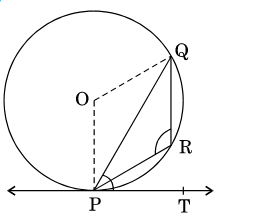
\includegraphics[width=\columnwidth]{figs/cbse_30_3_2.png}
	\label{Figure 2}
\end{figure}
\item The points 
\begin{align*}
 \vec{A}&= \myvec{4 \\ 7}\\  
 \vec{B}&=\myvec{p \\ 3}\\  
 \vec{C}&=\myvec{7 \\ 3}
\end{align*}
are the vertices of a right triangle, right-angled at $ \vec{B} $. Find the value of $p$.
\item In Figure \ref{Figure 3}, two tangents $RQ$ and $RP$ are drawn from an external point $R$ to the circle with centre $O$. If $\angle PRQ = 120 \degree,$ then prove that $OR = PR + RQ$.
  \begin{figure}[h!]
	\centering
    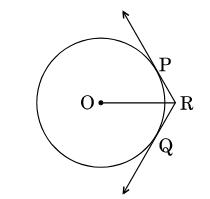
\includegraphics[width=\columnwidth]{figs/cbse_30_3_3.png}
	\label{Figure 3}
\end{figure}
\item In Figure \ref{Figure 4}, a triangle $ABC$ is drawn to circumscribe a circle of radius $3$ cm, such that the segments $BD$ and $DC$ are respectively of lengths $6$ cm  and $9$ cm. If the area of $\triangle \text{ABC is }54 cm^2$, then find the lengths of sides $AB$ and $AC$.
\begin{figure}[h!]
	\centering
    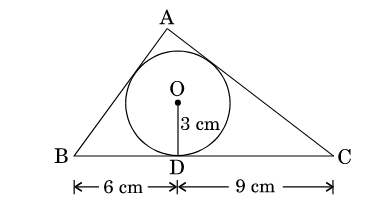
\includegraphics[width=\columnwidth]{figs/cbse_30_3_4.png}
	\label{Figure 4}
\end{figure}
\item Find the relation between x and y if the points 
\begin{align*}
\vec{A}&=\myvec{x \\ y}\\ 
\vec{B}&=\myvec{-5\\7}\\
\vec{C}&=\myvec{-4\\5} 
\end{align*}
are collinear.
\item Find the coordinates of a point $P$ on the line segment joining
\begin{align*}
\vec{A} &= \myvec{1\\2}\\
\vec{B} &= \myvec{6\\7}
\end{align*}
such that AP = $\dfrac{2}{5}$AB.
\item Find the values of $k$ for which the points
\begin{align*}
\vec{A} &= \myvec{k+1\\2k}\\
\vec{B} &= \myvec{3k\\2k+3}\\
\vec{C} &= \myvec{5k-1\\5k}
\end{align*}
are collinear.
\item Construct a triangle $ABC$ in which $AB = 5$ cm, $BC = 6$ cm and $\angle ABC = 60\degree$. Now construct another triangle whose sides are $\dfrac{5}{7}$ times the corresponding sides of $\triangle ABC$.
\item Prove that the lengths of the tangents drawn from an external point to a circle are equal.
\item Prove that the tangent drawn at the mid-point of an arc of a circle is parallel to the chord joining the end points of the arc.

\end{enumerate}
